\chapter{Verigraph}\label{ch:verigraph}

Verigraph is a new tool for simulating and verifying graph grammars, implemented in the purely functional programming language Haskell\footnote{The source code is available at \url{https://github.com/Verites/verigraph}}. The tool was designed aiming to be used as both an implementation of standard constructions and analysis for graph grammars and a sandbox for new ideas and techniques in graph grammars and other category theory related topics~\cite{BezerraETMF2016,Costa2016,CostaETMF2016, Becker2014}.

Regarding category theory, verigraph implements important basic constructions such as coequalizers, coproducts and colimits, pushout complements, initial pushouts, pullbacks, negative application conditions and constraints, among others.

The implemented categorial constructions are used as basis to implement several graph grammar analyses, such as critical pair analysis~\cite{Lambers2006}, state space generation from graph grammars and model checking using computation tree logic~\cite{Becker2014}, concurrent rules generation~\cite{BezerraETMF2016}, higher-order graph transformations~\cite{Machado2015}. They were also used to implement the calculation of occurrence graph grammars, which will be explained in depth on
chapter~\ref{ch:process} and used for test case generation on chapter~\ref{ch:tests}.

The analyses algorithms are implemented in a generic functional style, having the advantage of being very close to the formal definitions, thus making it easier to reason about them and to inspect for correctness. In addition, verigraph benefits from a layered architecture (see Figure~\ref{fig:verigraph:layers} \tinytodo{update figure}) where it is easy to reuse the same algorithms for other categories different than \cat{TGraph_T}, as long as they implement the contracts defined by the type classes (interfaces) defined on the system. Some examples of such type classes are show on
Figures~\ref{fig:verigraph:morphism-type-class} and \ref{fig:verigraph:cocomplete-type-class}.

\begin{figure}[!ht]
  \centering
  \fbox{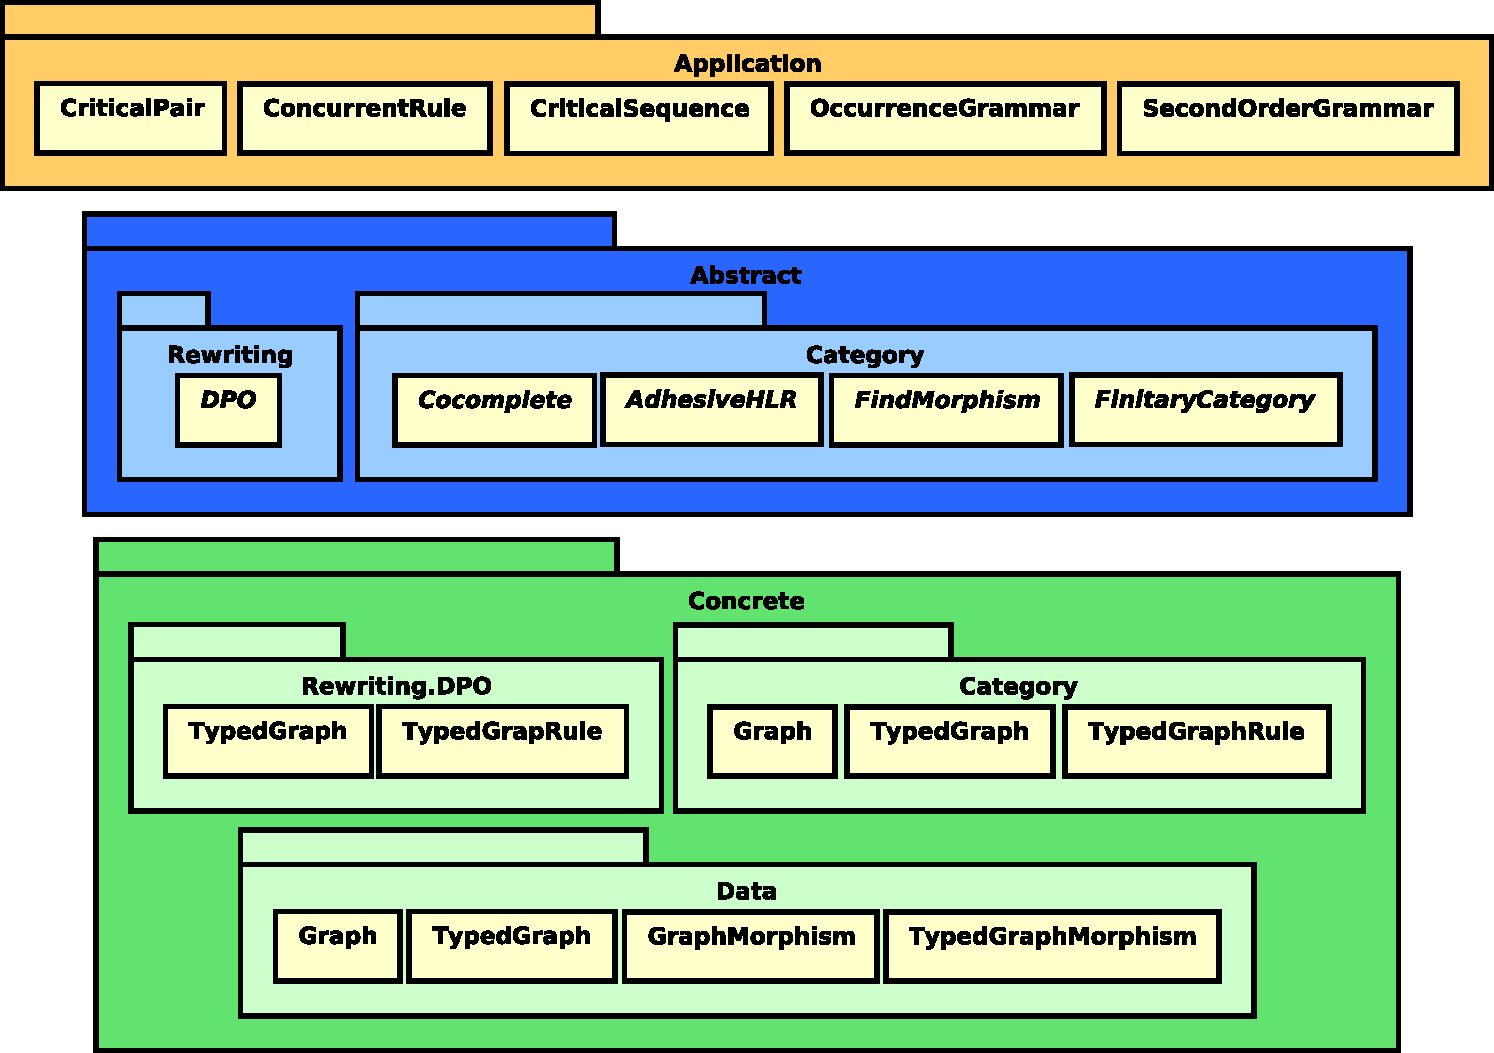
\includegraphics[scale=0.3]{images/verigraph/layers}}
  \caption{Verigraph layers: analyses algorithms (top layer), abstract categorial constructions (middle layer) and concrete categories (bottom layer).}\label{fig:verigraph:layers}
\end{figure}

There exist tools for analysing graph grammars which are similar to verigraph in some aspects, such as AGG~\cite{Taentzer2000} and GROOVE~\cite{Rensink2004}. However, to our knowledge, Verigraph is the only tool that integrates static and dynamic analyses, second-order specifications and provides support for new categorial constructions and algorithms, besides being the only tool in this field implemented in a pure functional language~\cite{Costa2016}.

\section{Categorial Constructions}

The first basic type class in Verigraph is \code{Morphism}, shown in Figure~\ref{fig:verigraph:morphism-type-class}, which serve as the minimal contract for every Category to be implemented in the tool. Notice how the contract of this type class reflects the category definition (see Definition~\ref{def:category}).

\begin{figure}[!ht]
\caption{Morphism Type Class}
\begin{minted}[linenos=true, breaklines,fontsize=\small]{haskell}
class (Eq m) => Morphism m where
    type Obj m :: *
    compose  :: m -> m -> m
    domain   :: m -> Obj m
    codomain :: m -> Obj m
    id       :: Obj m -> m
    isMonomorphism :: m -> Bool
    isEpimorphism :: m -> Bool
    isIsomorphism :: m -> Bool
\end{minted}
\label{fig:verigraph:morphism-type-class}
\end{figure}

All the other type classes related to category theory are somehow defined in terms of the \code{Morphism}. For example, the \code{Cocomplete} type class (shown in Figure~\ref{fig:verigraph:cocomplete-type-class}) defines some of the most basic categorial constructions used in verigraph, such as coequalizers and coproducts.

Notice that any category that implements the functions \code{calculateCoequalizer} and \code{calculateCoproduct} automatically has a standard implementation of the \code{calculatePushout} function based only on this two constructions. Furthermore, whenever a category has coequalizers and coproducts, it is possible to calculate any (finite) colimit based only on this two constructions, as demonstrated in~\cite{Pierce1991}.

\begin{figure}[!ht]
  \begin{minted}[linenos=true, breaklines, fontsize=\small]{haskell}
class (Morphism m) => Cocomplete m where

-- | Given two morphisms @/f : A -> B/@ and @/g : A -> B/@ returns the coequalizer morphism
-- @/h : B -> X/@
calculateCoequalizer :: m -> m -> m

-- | Given a non-empty list of morphisms of the form @/f : A -> B/@ returns the coequalizer Morphism
-- @/h : B -> X/@
calculateNCoequalizer :: NonEmpty m -> m

-- | Given two objects @A@ and @B@ it returns the coproduct @(A+B, f: A -> A+B, g: B -> A+B)@
calculateCoproduct :: Obj m -> Obj m -> (m,m)

-- | Given a non-empty list of objects @Bi@ it returns the coproduct @fi : Bi -> SUM(Bi)@
calculateNCoproduct :: NonEmpty (Obj m) -> [m]

calculatePushout :: m -> m -> (m, m)
calculatePushout f g = (f', g')
  where
    b = codomain f
    c = codomain g
    (b',c') = calculateCoproduct b c
    gc' = compose g c'
    fb' = compose f b'
    h = calculateCoequalizer fb' gc'
    g' = compose b' h
    f' = compose c' h
\end{minted}
\caption{Cocomplete Type Class}\label{fig:verigraph:cocomplete-type-class}
\end{figure}

Verigraph has several other important type classes, some examples are:
\begin{itemize}
  \item \code{FindMorphism} for finding morphisms between objects of a category;
  \item \code{AdhesiveHLR} for operations that AdhesiveHLR categories (e.g. \cat{TGraph_T}) are guaranteed to have such as calculating initial pushouts and pushout complements;
  \item \code{DPO} for operations related to DPO graph rewriting approach, such as inversion of rules.
\end{itemize}

Currently, there are three categories implemented on Verigraph: 

\begin{itemize}
  \item \cat{Graph}: graphs as objects and graph morphisms as arrows; 
  \item \cat{TGraph_T}: $T-$typed graphs as objects and $T-$typed graph morphisms as arrows; 
  \item \cat{T-Span}: $T-$typed graph morphism spans as objects and span morphisms as arrows (e.g. DPO graph rules and rule morphisms, respectively).
\end{itemize}

\section{Graph Grammar Constructions}

\begin{figure}[!ht]

\caption{Graph implementation}
\begin{minted}[linenos=true, breaklines,fontsize=\small]{haskell}
data Node a = Node 
{ getNodePayload :: Maybe a
} deriving (Show, Read)

data Edge a = Edge 
{ getSource      :: NodeId
, getTarget      :: NodeId
, getEdgePayload :: Maybe a
} deriving (Show, Read)

data Graph a b = Graph 
{ nodeMap :: [(NodeId, Node a)]
, edgeMap :: [(EdgeId, Edge b)]
} deriving (Show, Read)
\end{minted}
\end{figure}

\begin{figure}[!ht]
\caption{Different Implementations of the Morphism Type Class}
\begin{minted}[linenos=true, breaklines,fontsize=\small]{haskell}
data GraphMorphism a b = GraphMorphism 
{ getDomain    :: Graph a b
, getCodomain  :: Graph a b
, nodeRelation :: R.Relation G.NodeId
, edgeRelation :: R.Relation G.EdgeId
} deriving (Eq, Show)

-- | A typed graph is a morphism whose codomain is the type graph.
type TypedGraph a b = GraphMorphism a b

data TypedGraphMorphism a b = TypedGraphMorphism 
{ getDomain   :: TypedGraph a b
, getCodomain :: TypedGraph a b
, mapping     :: GraphMorphism a b
} deriving (Eq, Show)

data RuleMorphism a b = RuleMorphism 
{ rmDomain         :: Production (TypedGraphMorphism a b)
, rmCodomain       :: Production (TypedGraphMorphism a b)
, mappingLeft      :: TypedGraphMorphism a b
, mappingInterface :: TypedGraphMorphism a b
, mappingRight     :: TypedGraphMorphism a b
} deriving (Eq, Show)
\end{minted}
\end{figure}

\begin{figure}[!ht]
\caption{Typed graph morphism implementation of the morphism type class.}
\begin{minted}[linenos=true, breaklines,fontsize=\small]{haskell}
instance Morphism (TypedGraphMorphism a b) where
  type Obj (TypedGraphMorphism a b) = TypedGraph a b
  domain = getDomain
  codomain = getCodomain
  compose t1 t2 = TypedGraphMorphism (domain t1) (codomain t2) $ compose (mapping t1) (mapping t2)
  id t = TypedGraphMorphism t t (M.id $ domain t)
  isMonomorphism = isMonomorphism . mapping
  isEpimorphism = isEpimorphism . mapping
  isIsomorphism = isIsomorphism . mapping

\end{minted}
\end{figure}

\begin{figure}[!ht]
\caption{Delete-Use and Produce-Use Implementation}
\begin{minted}[linenos=true, breaklines,fontsize=\small]{haskell}
-- | Rule @p1@ is in a delete-use conflict with @p2@ if @p1@ deletes something that is used by @p2@. This function verifies the non existence of h21: L2 -> D1 such that d1 . h21 = m2
isDeleteUse :: DPO m => Production m -> (m, m) -> Bool
isDeleteUse p1 (m1,m2) = null h21
  where
    --gets only the morphism d1 from D1 to G
    (_,d1) = calculatePushoutComplement m1 (getLHS p1) 
    h21 = findAllPossibleH21 m2 d1

isProduceUse :: DPO m => Production m -> (m, m) -> Bool
isProduceUse p1 (m1',m2) = null h21
  where
   --gets only the morphism d1 from D1 to G
   (_,e1) = calculatePushoutComplement m1' (getRHS p1)
   h21 = findAllPossibleH21 m2 e1
\end{minted}
\end{figure}


